% \begin{itemize}
%     \item What is a porous material? 
%     \begin{itemize}
%         \item What makes them different to non-porous materials?
%         \item Why do their differences make them industrially relevant?
%         \item What are some synthesis techniques that exist?
%         \item What are weaknesses with those synthesis techniques?
%     \end{itemize}
%     \item What is a particle stabilized emulsion
%     \begin{itemize}
%         \item Why are they interesting for porous material applications?
%         \item What is a bijel?
%         \item How are bijels relevant to porous materials?
%         \item Fabrication techniques that are proposed which allow large scale bijel fabrication
%         \item microstructure control in those applications
%     \end{itemize}
%     \item Purpose of study
%     \begin{itemize}
%         \item Three aims of the study 
%         \item significance of study
%         \item assumptions and limitations of the study
%     \end{itemize}
%     \item Summary of motivation, purpose and research aims
% \end{itemize}

% \textcolor{blue}{
% \begin{itemize}
%   \item Explain what is a porous material and the advantages they have in their applications compared to non-porous materials 
%   \item Detailed description of their applications and why we are interested in stimuli responsive porous materials 
%   \item Overview of porous material synthesis techniques and what are some areas where there is room for improvement (Definition of critical issues)
%   \item Explain what emulsion templating is and the specific advantages it has over other techniques. Recall where it has been used to great effect
%   \item Explain how bijels fit into emulsion templating and how they offer advantages to standard emulsion templates
%   \item Explain how bijels have been manufactured
%   \item Linking stimuli response as a way to add additional functionality to bijels and identifying how to process them more effectively
%   \item Explain why magnetic fields are interesting in this case
%   \item Explain what is a bijel, how they have been synthesized and some hints at past work for controlling their microstructure (literature review)
%   \item Explain how bijels and stimuli response can address the shortcomings addressed in the previous section (Research objectives)
% \end{itemize}
% }

\section{Introduction}
\label{section:introduction}

Porous materials are characterized by the presence of pores or voids within their structure, where no solid material is present. 
In contrast, homogeneous materials exhibit a uniform structure devoid of pores. The shape and distribution of these pores can vary, 
and according to the IUPAC classification, materials are categorized based on pore size as microporous ($L < 2$ nm), 
mesoporous ($2 < L < 50$ nm), or macroporous ($L > 50$ nm) \cite{sing_reporting_1985}. The presence of pores significantly 
increases the surface area-to-volume ratio of porous materials compared to their homogeneous counterparts. A commonly used experimental 
technique for estimating the surface area of porous materials, based on Brunauer-Emmett-Teller (BET) theory, has demonstrated that such 
materials can exhibit surface areas more than a hundred times greater than those of homogeneous materials, depending on pore size and pore 
size distribution \cite{shimizu_surface_2022}.  

In addition to pore size and its distribution, the spatial arrangement of pores within a material significantly influences its performance, 
often quantified by tortuosity. Tortuosity is defined as the ratio of the actual path length between two points to the Euclidean distance 
between them. A tortuosity greater than one indicates that the path length is longer than the Euclidean distance, whereas a tortuosity less 
than one suggests a more direct pathway. The interplay of these factors has led to the development of a wide range of tailored microstructures 
for diverse applications. Each pore size regime serves distinct functions; for example, microporous materials are commonly used in zeolites and 
photonic bandgap materials, while macroporous materials enhance transport properties, making them suitable for applications such as battery 
electrodes and drug delivery systems \cite{chen_tortuosity_2020, ebner_tortuosity_2014}. The increased surface area-to-volume ratio of porous 
materials further enhances the properties of the base material in various applications, including catalysis, energy storage, and biomedical 
systems, making them important microstructures. \cite{cha_bicontinuous_2019, samdani_bicontinuous_2017, thorson_bijel-templated_2019, zhao_highly_2014}.  

\begin{figure}
    \centering
    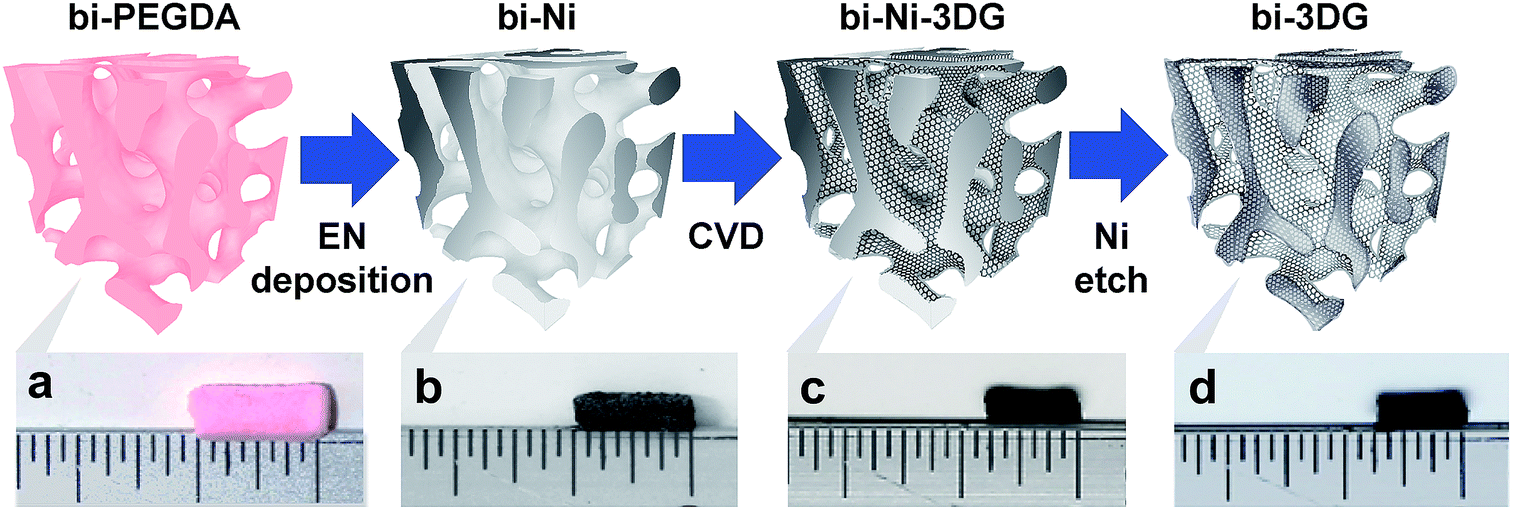
\includegraphics[scale = 0.5]{figures/introduction/bijel_templating.png}
    \caption{Fabrication of a graphite oxide battery electrode using bijel template. Reproduced from Garcie et al. under license number 1548092-1. \cite{garcia_scalable_2019}}
    \label{fig:bijel_template}
\end{figure}

Conventionally, porous materials have been synthesized through methods such as solvothermal synthesis and pyrolysis, which are commonly 
used for producing zeolites and activated carbon, respectively. With the increasing demand for tailored porous materials, advanced synthesis 
techniques—including sol-gel synthesis, freeze-drying, and various templating methods—have been developed to fabricate porous structures across 
length scales ranging from $10^{-9}$ m to $10^{-3}$ m 
\cite{stein_morphological_2008, ray_comprehensive_2016, cervellere_mesoscopic_2019, garcia-bennett_unique_2020, zhang_emulsion_2019, alves-rosa_design_2013}. 
Industry has also adopted techniques such as electro-spinning to produce nonwoven fibers, which are widely used in membrane synthesis.  
Among these approaches, templating techniques provide precise control over pore size, enable bottom-up synthesis, and introduce functionality by 
leveraging various physical phenomena. Colloidal templating relies on the close packing of particles to define pore structures. Surfactant and 
polymer templating utilize the self-assembly of macromolecules into their equilibrium configurations to generate porous networks. Emulsion templating, 
on the other hand, exploits the phase separation of partially miscible liquids to form the pore architecture of the resulting material.  

Emulsion templating enables the fabrication of porous materials with a wide range of tunable pore sizes, continuous production through microfluidic 
junctions or other flow-based systems, and functionalization through the incorporation of additives or stabilizers. This technique also offers a broad 
scope of accessible microstructures and benefits from mild synthesis conditions. Additionally, it can be extended to generate hierarchical porosity, 
further enhancing the functionality and properties of the resulting materials \cite{yang_hierarchically_2017, thompson_hierarchically_2019, wang_morphology_2023}.  
Figure \ref{fig:bijel_template} illustrates how emulsion templating enables the bottom-up synthesis of hierarchically porous materials, although various 
alternative approaches also exist 
\cite{garcia_scalable_2019, santiago_cordoba_aerobijels_2020, thorson_bijel-templated_2019, lu_controllable_2020, wang_morphology_2023}.

\begin{figure}
    \centering
    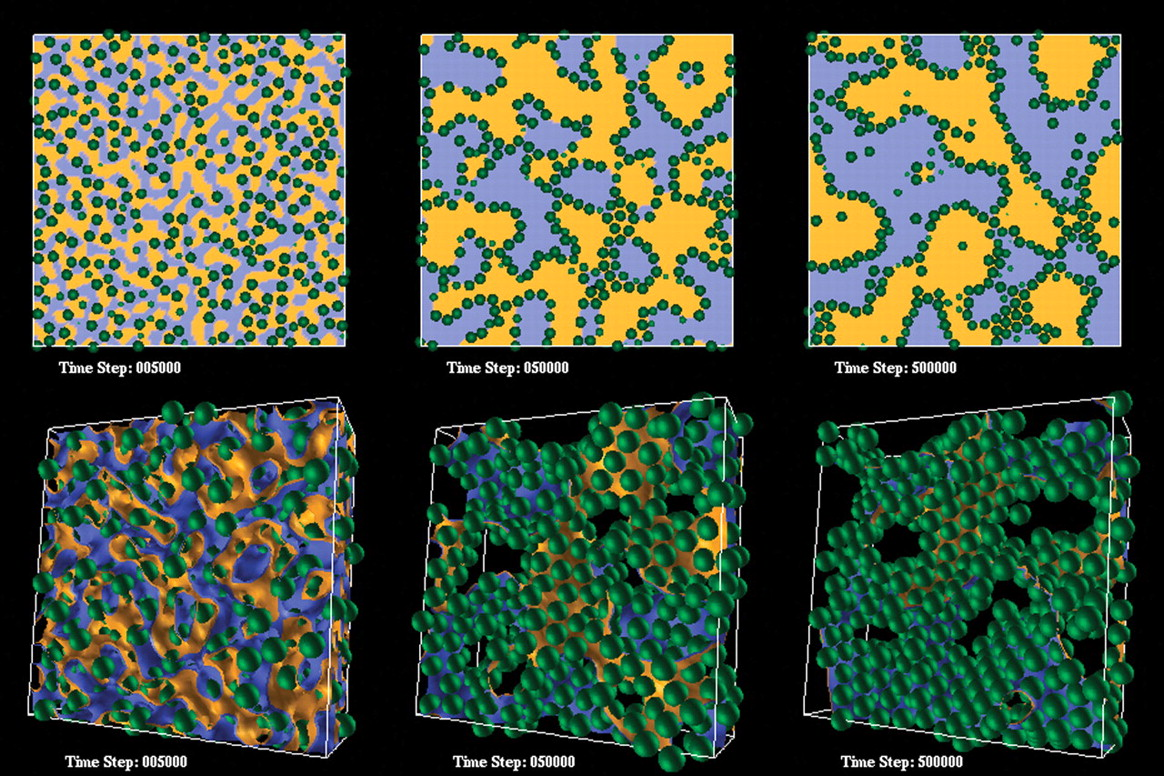
\includegraphics[scale = 0.3]{figures/introduction/bijel_coarsening.jpg}
    \caption{Initiation and arrest of spinodal decomposition as particles adsorb onto the interface, followed by jamming once the 
    interfacial area matches the cross sectional area of the adsorbed particles\cite{stratford_colloidal_2005}. Reproduced from Adhikari et al. 
    under license number 5966820525314.}
    \label{fig:bijel_coarsen}
\end{figure}

One particularly interesting emulsion-derived microstructure is the bicontinuous interfacially jammed emulsion gel (bijel) 
\cite{stratford_colloidal_2005, herzig_bicontinuous_2007, lee_bicontinuous_2010}. Bijels are formed by arresting the spinodal decomposition of partially 
miscible liquids, a process driven by the adsorption of colloidal particles at the interface. As the interfacial area contracts, the particles become 
jammed, stabilizing the bicontinuous structure, as summarized in Figure \ref{fig:bijel_coarsen}. The resulting co-continuous and tortuous microstructure 
of bijels makes them highly suitable for various porous material applications.  

Bijels were first predicted in simulations in 2005 and experimentally realized in 2007 when a mixture of water and 2,6-lutidine, combined with 
surface-modified silica nanoparticles, underwent thermally induced spinodal decomposition \cite{stratford_colloidal_2005, herzig_bicontinuous_2007}. 
Since then, various casting mixtures and particle chemistries have been explored to fabricate bijels using thermally induced spinodal decomposition (TIPS) 
\cite{lee_bicontinuous_2010, bai_dynamics_2015}. More recently, alternative fabrication techniques such as solvent transfer-induced phase separation (STrIPS), 
vapor-induced phase separation (VIPS), non-solvent-induced phase separation (NIPS), homogenization, and liquid-in-liquid printing have been developed. 
These methods enable the continuous synthesis of bijels, making them more suitable for large-scale production 
\cite{haase_continuous_2015, wang_scalable_2020, cai_bijels_2017, yabuno_preparation_2020, wang_bicontinuous_2023, amirfattahi_fabrication_2024}. 
Additionally, these techniques allow for the fabrication of bijels in various shapes and form factors, including fibers, coatings, and capsules, expanding 
their applicability across different fields, as illustrated in Figure \ref{fig:strips} 
\cite{haase_continuous_2015, boakye-ansah_controlling_2020, kharal_hightensile_2020, wang_bicontinuous_2023}.  

\begin{figure}[h]
    \centering
    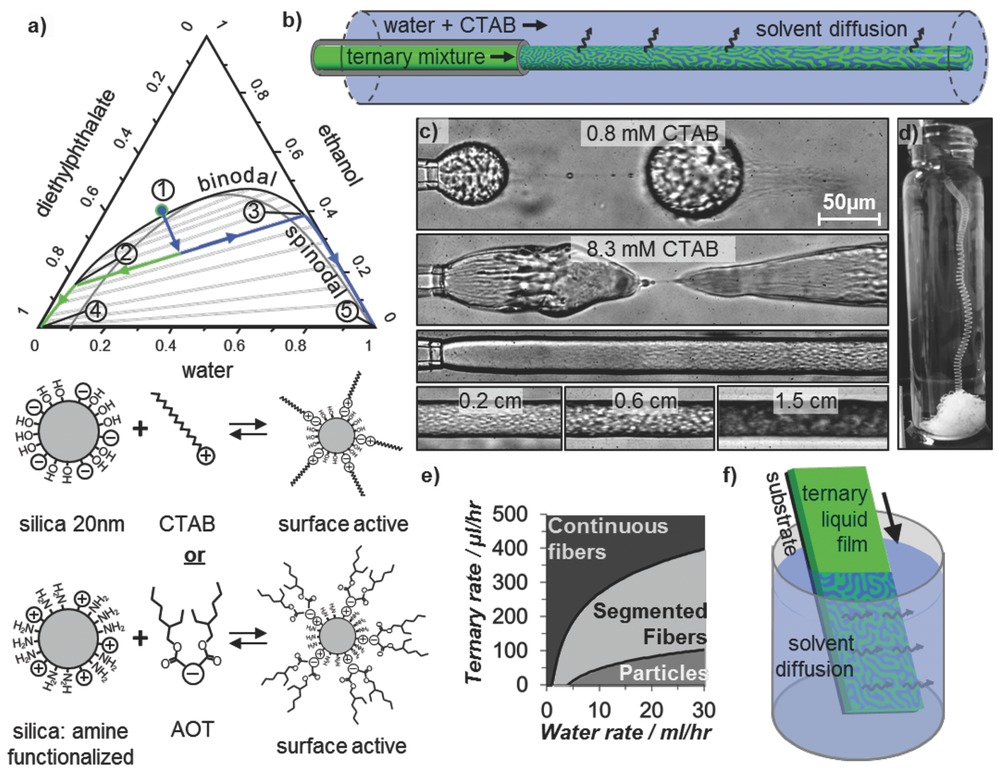
\includegraphics[scale = 4]{figures/introduction/STrIPS.jpg}
    \caption{STrIPS in action. Extrusion of the bijel casting mixture into a non-solvent bath, followed by removal of solvent from 
    the casting mixture through diffusion. Reproduced from Haase et al. 2015 under license number 5913140219015. \cite{haase_continuous_2015}}
    \label{fig:strips}
\end{figure}

However, all of these techniques rely on precisely controlling the rate of phase separation, which typically involves adjusting the composition 
of the casting mixture to modify the resulting microstructure. In STrIPS, for example, the bijel microstructure is influenced by both the flow rate 
and the choice of co-solvent, which are selected to regulate the phase separation dynamics \cite{haase_continuous_2015}. These factors directly 
impact material properties such as the mechanical stability of the bijel, which is particularly important in applications like catalysis, where the 
rigidity of the particle monolayer is essential for maintaining consistent performance 
\cite{reeves_particle-size_2015, haase_situ_2016, boakye-ansah_controlling_2020}. Identifying alternative techniques for modifying the microstructure of 
bijels would allow for greater tunability while maintaining the desired composition of the constituent materials. One promising approach for achieving 
such control is the use of stimuli-responsive mechanisms.  

\begin{figure}[h]
    \centering
    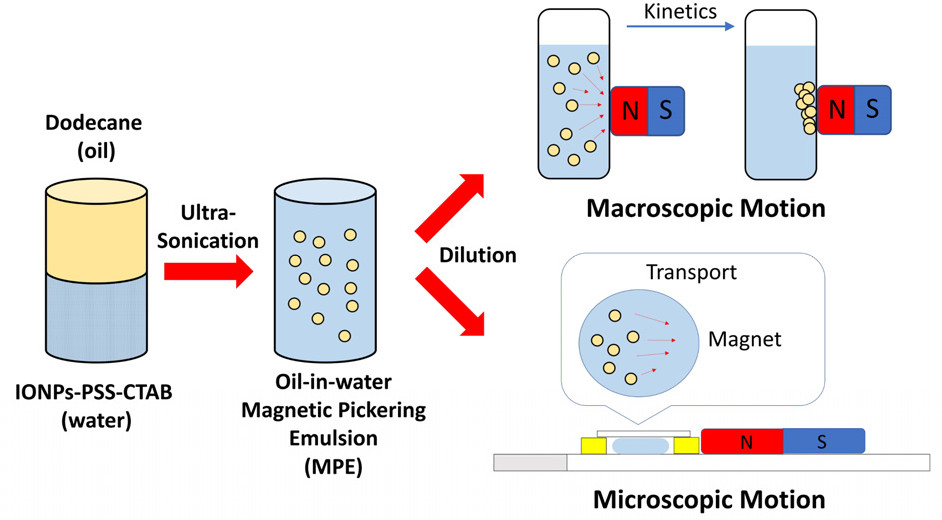
\includegraphics[scale = 1]{figures/introduction/magnetophoresis_emulsion.jpeg}
    \caption{Enhanced oil recovery of oil from water using magnetically responsive emulsion stabilizers, allowing for 
             locomotion and controlled coalescence of cargo from a matrix phase using magnetic fields relevant in 
             water filtration and oil refining applications. Reproduced from Tham et al. 2021 under the ACS standard license \cite{tham_magnetophoresis_2021}}
    \label{fig:magnetophoresis_droplet}
\end{figure}

Stimuli-responsive mechanisms based on pH, external fields, and temperature have been explored in previous studies to modify the microstructure of emulsion 
droplets for applications such as enhanced oil recovery, pharmaceuticals, and cell adhesion 
\cite{haase_nanoparticle_2011, tham_magnetophoresis_2021, cui_stabilizing_2013, manfredini_limonene--water_2021}. External fields have been shown to 
manipulate emulsion stability, control droplet movement, and induce elongation in emulsion droplets 
\cite{tham_magnetophoresis_2021, cui_stabilizing_2013, melle_pickering_2005}. One such example is shown in Figure \ref{fig:magnetophoresis_droplet}
where enhanced oil recovery was performed using magnetically responsive particle stabilizers which could capture oil droplets,
move the droplets away from the matrix and cause controlled coalescence elsewhere.
In the case of bijels, spherical particle-stabilized systems subjected to a magnetic field exhibited no significant microstructural changes 
\cite{kim_bijels_2010}. However, bijels stabilized with spherical particles under an electric field demonstrated greater potential for microstructure 
modification \cite{carmack_tuning_2018}. Despite this, magnetic fields present a promising avenue for targeted stimuli-responsive behavior, as even 
weak fields can induce a response while remaining non-invasive in many contexts. This property is particularly advantageous for pharmaceutical and 
bioengineering applications, where external control over material properties is desirable 
\cite{vanoli_bijels_2022, thorson_bijel-templated_2019, thorson_composite_2018}.  
Such applications could benefit from in-situ microstructural modifications, enabling tunable drug delivery rates, improved separations, and enhanced catalyst 
efficiency and permeability. Therefore, developing strategies to modify pore size and tortuosity without requiring the synthesis of a new material would 
significantly expand the functional versatility of bijels.  

\begin{figure}[h]
    \centering
    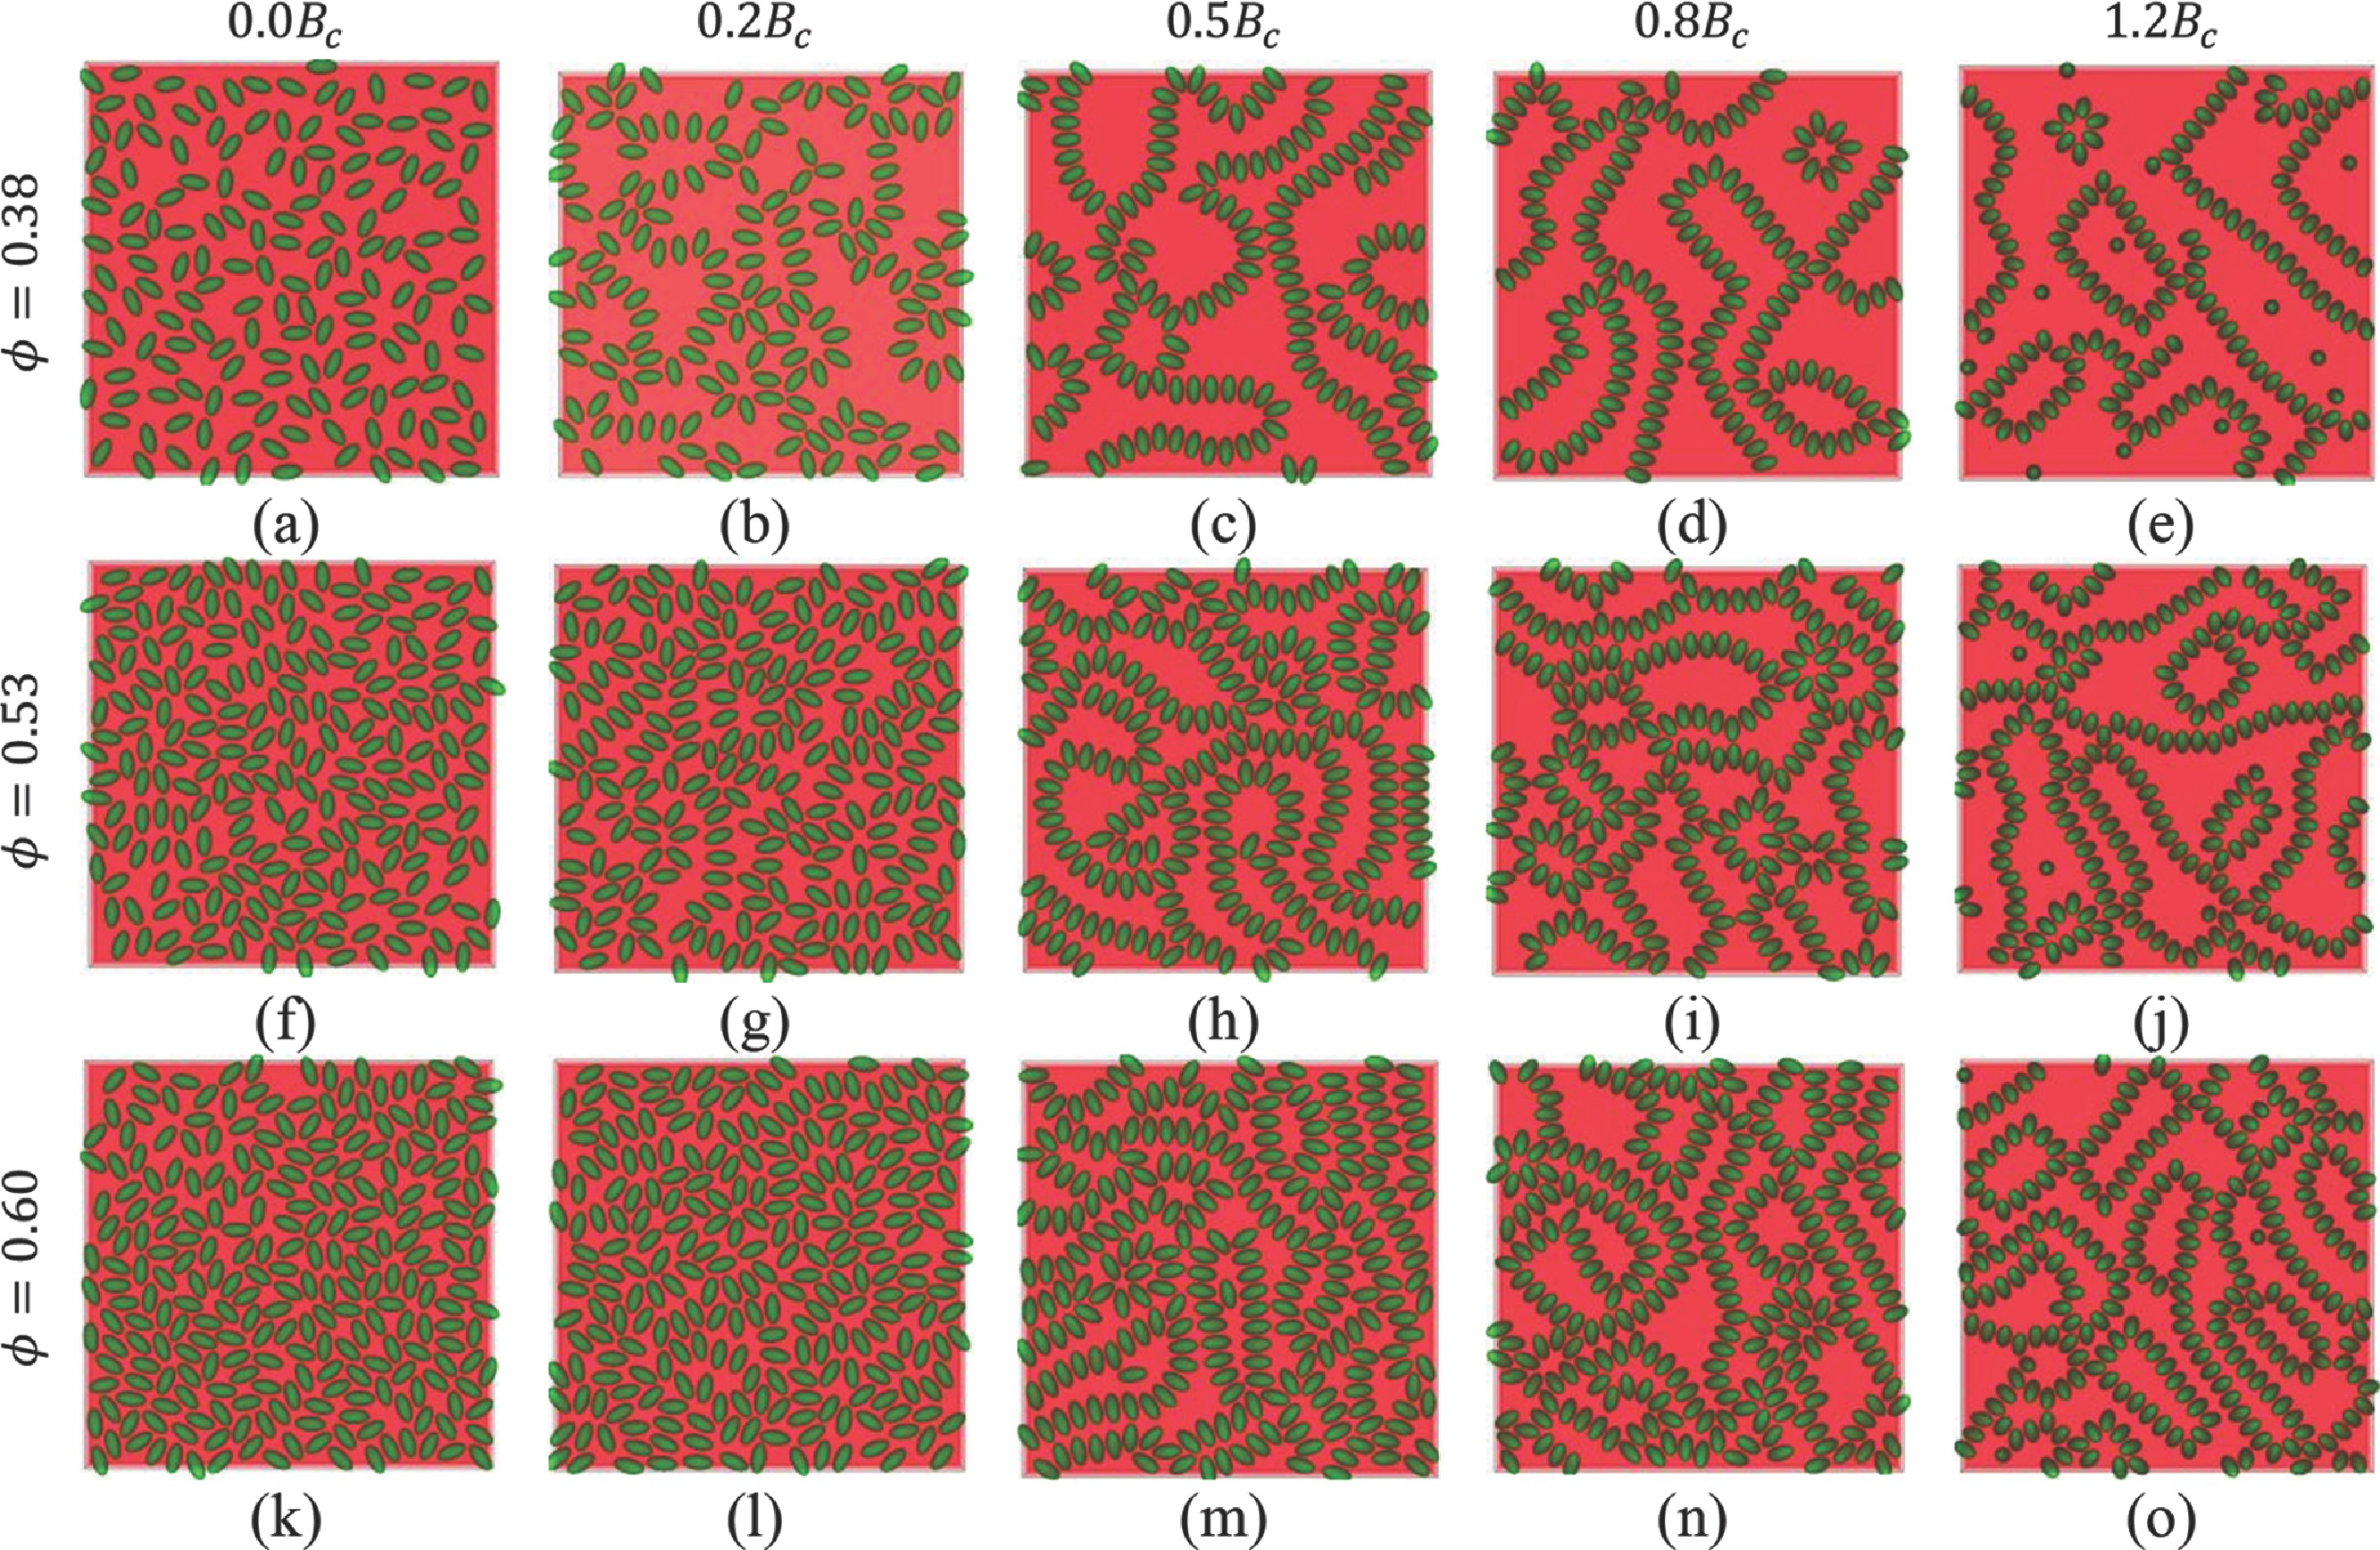
\includegraphics[scale = 0.4]{figures/introduction/anisotropic_particles_assembly.jpg}
    \caption{Assembly of prolate particles on a flat interface at various interfacial coverages and field strengths,
             showing the self assembly into chains that ellipsoidal particles can undergo under applied magnetic fields at
             interfaces. Reproduced from Davies et al. under the Creative Commons CC BY license \cite{davies_assembling_2014}}
    \label{fig:anisotropic_assembly}
\end{figure}

Anisotropic particles at interfaces have been shown to undergo self-assembly due to the presence of multipolar pressure fields induced by interface 
deformation caused by magnetic stimuli, visualized in Figure \ref{fig:anisotropic_assembly}. \cite{bresme_orientational_2007, davies_interface_2014}
When subjected to a magnetic field, assemblies of multiple ellipsoidal particles exhibit energy minima at orientations different from those of isolated 
particles. This suggests that the interfacial coverage of surfaces decorated with ellipsoidal particles can be dynamically tuned using external 
stimuli \cite{newton_influence_2014, newton_capillary_2018}. Therefore, ellipsoidal particles at interfaces—whose orientation and packing can be externally 
controlled—present a promising strategy for tailoring the microstructure of bijels.  

Bijels offer a bottom-up synthesis approach for porous material templates, enabling scalable and continuous fabrication for both hard and soft material 
applications through STrIPS and related techniques. However, the degree of microstructural control provided by these methods is inherently dependent on 
the composition of the casting mixture. Stimuli-responsive strategies present a means to modify the microstructure of bijels while preserving the 
diverse form factors achievable through continuous synthesis techniques. Previous attempts to induce magnetic stimuli response in bijels stabilized 
with spherical particles have shown limited success \cite{kim_bijels_2010}.  

Building on this background, we propose the use of anisotropic particles as a technique to enable microstructure modification of bijels upon the application 
of an external field, both during and after fabrication. This work aims to explore methods for controlling the bijel microstructure independently of the casting 
mixture composition by utilizing magnetic stimuli on bijels stabilized with magnetically responsive ellipsoidal particles.  
The proposed mechanism of microstructure modification is based on the reorientation of particles in response to the applied magnetic field, which alters the 
packing arrangement of the particles at the interface. By modifying the interfacial packing, the point at which the particles jam is also altered, thereby 
affecting the jamming point of the bijel. This mechanism is expected to be effective both during and after the synthesis process. Additionally, the 
processability of bijels produced using this technique will be examined to assess how changes in particle packing influence the rheological properties of 
the material.  

\section{Research objective}

% this work seeks to identify means to control the bijel microstructure independent of the casting mixture composition utilizing magnetic stimuli response of anisotropic particles. The proposed mechanism of microstructure modification is driven through reorientation of the particles to the applied magnetic field altering how the particles pack on the interface.

\subsection{Aim 1: Determination of the degree of microstructure changes expected when applying a constant field during bijel formation}
\label{section:aim1_desc}

The jamming point of a bijel plays a crucial role in determining the resulting microstructure, as demonstrated by previous studies comparing the length scales 
of bijels synthesized with varying particle volume fractions and sizes \cite{jansen_bijels_2011, reeves_particle-size_2015}. Additionally, it has been shown 
that magnetic fields can facilitate the self-assembly of anisotropic particles at interfaces and control the interfacial angle between the particle's axis 
of symmetry and the interface \cite{davies_interface_2014, davies_assembling_2014}. However, on a curved interface with numerous other particles, it remains 
unclear how the orientation of multiple particles in response to the field and their regular arrangement will influence the jamming behavior of the bijel 
\cite{bresme_orientational_2007, davies_interface_2014}.  

To evaluate the microstructure obtained upon the application of a field during the formation of the bijel, homogeneous mixtures containing spherical and 
ellipsoidal particles will be subjected to field strengths both above and below the critical field strength. This critical field strength is the threshold 
at which particle orientations to the interface are governed by the applied field, as calculated by Bresme and Faraudo for the particle aspect ratio 
\cite{bresme_orientational_2007, davies_interface_2014}. The range of selected field strengths will provide insight into the mechanisms controlling 
microstructural changes, enabling verification of the hypothesis and identification of the conditions under which the most control over the microstructure 
can be achieved.

The average and directional domain sizes, along with their relationship to tortuosity, will be used to characterize the microstructural properties of the 
resulting bijel. The nematic order parameter and the average interfacial angle will provide insight into how the application of the field influences particle 
ordering, both among the particles and relative to the interface. Finally, the radial distribution function will be employed to assess whether the expected 
orientational changes upon field application affect the packing of particles at the interface.

\subsection{Aim 2: Microstructure changes and timescales upon application of a magnetic field after formation}
\label{section:aim2_desc}

Particles at the surface of emulsion droplets have been shown to unjam and rejam into new, stable microstructures upon the application of stimuli 
\cite{cui_stabilizing_2013}. Magnetic fields applied to bijels stabilized with ellipsoidal particles will promote the unjamming and rejamming of the 
particle monolayer, leading to modifications in the bijel's microstructure. Due to local changes in the state of the particles—specifically, alterations 
in the interfacial ordering and the direction and arrangement of particles—we anticipate that microstructure changes will persist even after the magnetic 
field is turned off. Two mechanisms for microstructure modification are proposed. The first suggests that the adsorption energy is sufficiently strong to 
cause the interface to move with the particles, allowing them to rejam in new locations and orientations relative to the field. The second mechanism posits 
that the particles tilt within the interface, leading to domain coarsening before jamming in their new positions and orientations. This study will assess the 
mechanism, the resulting microstructural changes, and the associated timescales.

The response of bijels to magnetic fields will be evaluated by analyzing how model bijels, synthesized without applied fields, respond to field 
strengths both above and below the critical field strength, as calculated using Bresme and Faraudo's theory. Microstructural properties, including the 
average domain size, particle orientation relative to the field and interface, and the Steinhardt 6-fold bond order parameter, will be used to examine 
the spatial relationships between particles and their neighbors. These techniques will enable the identification of the mechanisms active at different 
magnetic field strengths. Additionally, the observed microstructure changes will be characterized and compared to assess how the applied magnetic field 
influences the final microstructure.

Next, the importance of the initial ordering of the particle monolayer will be assessed by increasing the applied field to levels equal to the surface 
tension forces on bijel templates simulated under various field strengths. The applied field will also be switched off for bijel templates simulated under 
the same conditions. The same analysis metrics mentioned previously will be used. Additionally, microstructures with the same difference in applied field 
will be examined to investigate the reversibility of bijel microstructures.

\subsection{Aim 3: Rheological characterization of bijels formed under and subjected to a magnetic field}
\label{section:aim3_desc}

In many of the fabrication processes described above, the rheology of the bijel casting mixture plays a crucial role 
\cite{haase_continuous_2015, cai_bijels_2017, amirfattahi_fabrication_2024}. Furthermore, the mechanical performance of the
resulting bijel is a key constraint for bijels in cross flow reactors or water filtration applications. \cite{boakye-ansah_controlling_2020}
Under high shear, the bijel can fail due to particles being ejected from the interface limiting the flow rate and pressure that can
be used when using bijels as cross flow reactors or water filtration systems. Ching demonstrated that, rheologically, bijels behave 
as colloidal glasses percolating in 3D space \cite{ching_bijel_2022}. This implies a yield stress above which flow of the material
will initiate. Bijels are also shear thinning as fluid-particle interactions increase the effective viscosity at lower shear rates.


% $Ca_s = \frac{\eta_{f} \dot{\gamma} L_{1}}{\sigma}$ where $\dot{\gamma} = \frac{u_{LE}}{L_x}$ is the strain rate and 
% $L_1$ is the average domain size. \cite{frijters_effects_2012, yang_capillary_2022} Lower capillary numbers in the range of
%  $ 10^{-7} \geq Ca_s \leq 10^{-5}$ will be utilized. 
% which corresponds to a $Ma << 0.01$ to accommodate the hydrodynamic model utilized.

In this study, the yield stress and viscosity of the bijels will be examined as a function of the initial microstructure under various $Ca_s$ values. 
A shear capillary number, $Ca_s$, is defined to correlate the applied strain rate with the capillary forces derived from surface tension 
\cite{frijters_effects_2012, yang_capillary_2022}. This study aims to identify the effect 
of the initial microstructure and applied field on the rheological properties of the bijel.The initial microstructure will be 
derived from bijels stabilized with ellipsoidal particles, synthesized both without a magnetic field and with a field 
strength equal to the surface tension energy. Constant shear, defined by $Ca_s$, will be applied to determine the yield stress and non-Newtonian 
characteristics of the bijel. Previous studies have shown that particle ordering in the direction of shear significantly alters the rheological behavior 
compared to unordered systems. Additionally, the domains within the bijel may introduce new mechanisms for modifying rheological properties, which have 
yet to be explored in detail.

% We will then investigate the complex rheology of the bijels by calculating the loss and storage moduli of the bijel microstructures described 
% earlier as a function of oscillatory shear. The loss and storage moduli describe the viscous and elastic behavior of the bijel, respectively, 
% allowing the gel point of the bijel to be determined as the point at which the storage modulus exceeds the loss modulus. Special attention will be 
% given to the state of the particles in all simulations, correlating changes in particle properties with observed rheological events. Additionally, 
% we will assess whether shear banding occurs.